\label{sec:architecture}

This section describes how the different components of the system are
composed to build a coherent piece. A complete diagram of the
architecture can be seen in \cref{fig:architecture}.

The system is separated in two main parts: a client and a server. The
client is simpler than the server; its main task is to display
information given by the server, and can therefore be seen as a dumb
client. All the business logic is contained on the
server. This communication occurs through the \textit{system interface}
components of the client and server. The information being sent back and
forth between the client and server is displayed in the \textit{user interface}
component of the client and the server.

The aforementioned business logic on the server is a collection of
many different components. Each of these components have a distinct
responsibility. For example, the \textit{UserService} has the responsibility to
handle all actions related to users of the application. The
\textit{UserService} component defines the functions involving users. It is
therefore placed in the function layer of the server. To perform its
actions, the \textit{UserService} component has associations to the \textit{User}
component defined in the model layer of the server.

Another layer of the server architecture is the
technical platform. Components contained in this layer are all
libraries defined outside of the business logic of the server, but are
still as part of the complete system. For example, the
\textit{SpotifyDotNet} component is a library for streaming tracks from
Spotify. The implementation of this library is described in
\cref{imp:libspotify}.

\begin{figure}
  \centering
  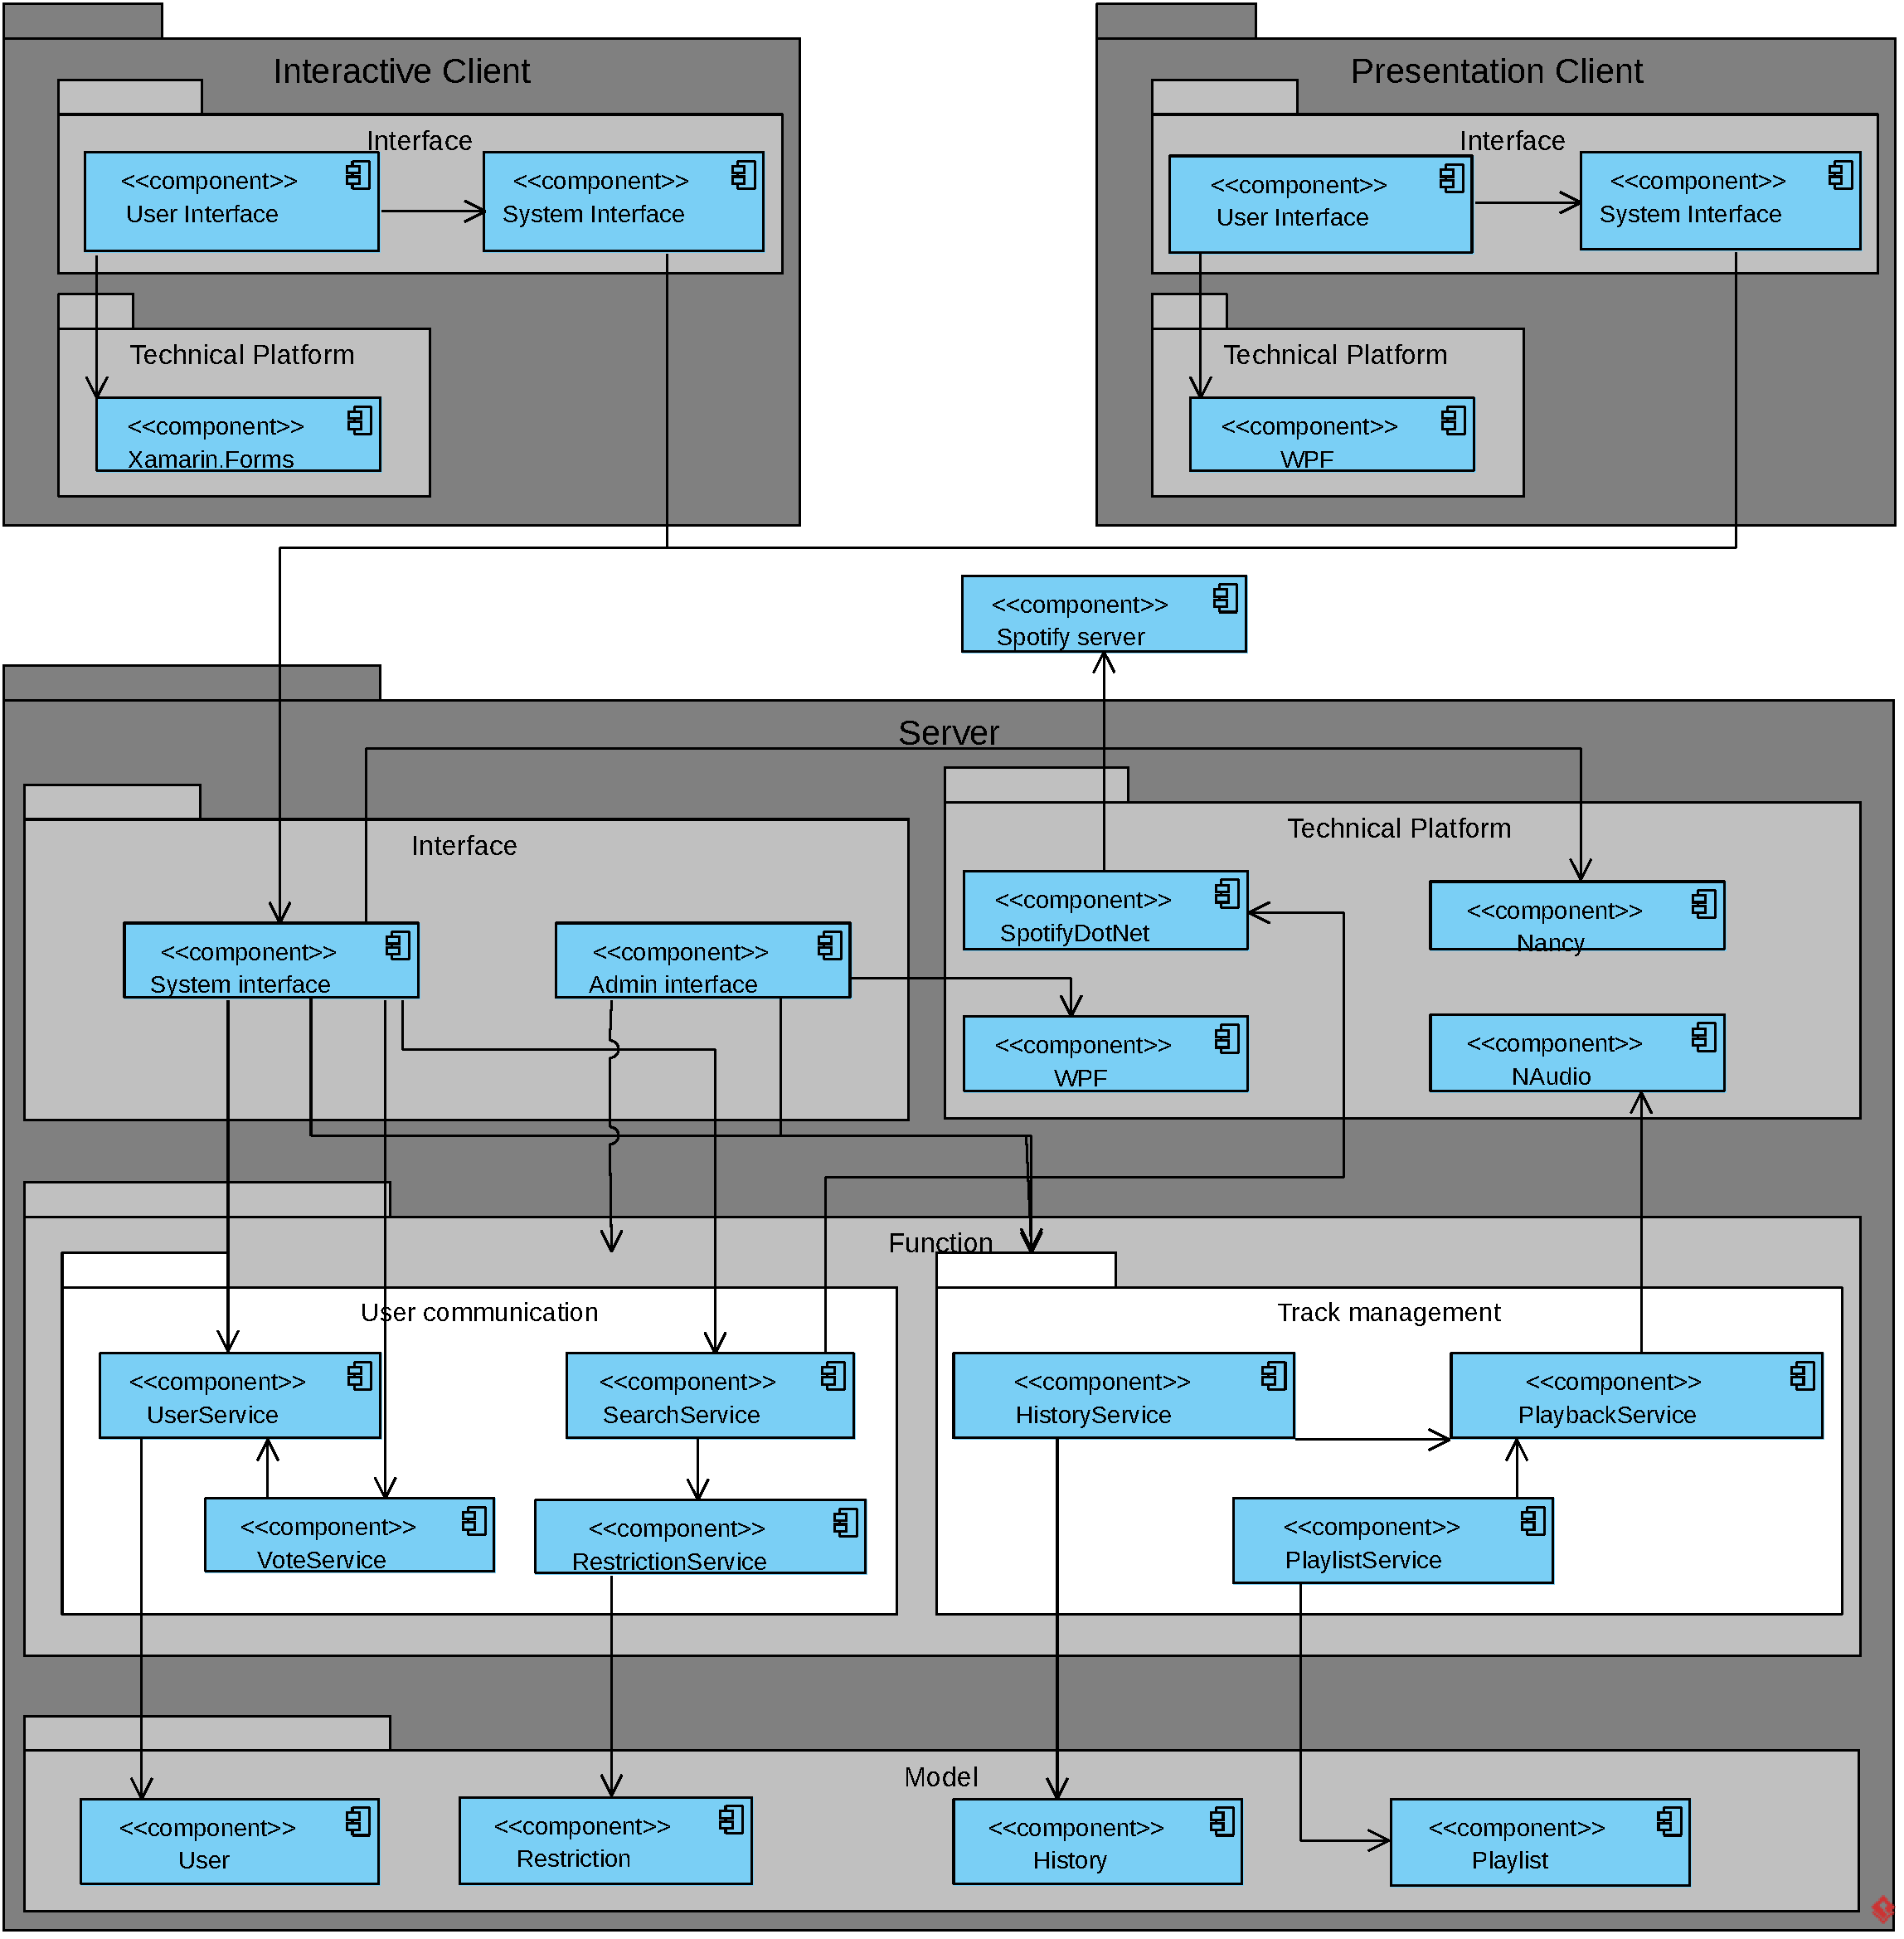
\includegraphics[width=1.2\linewidth]{Images/Arkitektur.pdf}
  \caption{Architecture of the system}\label{fig:architecture}
\end{figure}
